% ---------------------------------------------------------------- 23 Nov 2026: FairShip full-Geant4 cross-check (noSBT_full)
\begin{btframe}{7 · Back-up · FairShip cross-check}{FairShip full Geant4 vs our chain: MS7 production and cavern tracks at SST1}
\noindent \begin{minipage}[t]{\dimexpr(0.47\linewidth-0.47\dimexpr9.67pt\relax)}\vspace{0pt}\centering
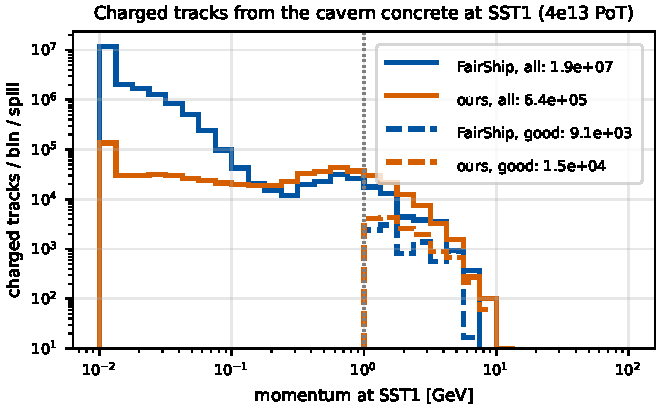
\includegraphics[width=\linewidth,height=150pt,keepaspectratio]{figs/s45_fairship_cavern_p.pdf}\par
\end{minipage}%
\hfill%
\begin{minipage}[t]{\dimexpr(0.53\linewidth-0.53\dimexpr9.67pt\relax)}\vspace{0pt}\raggedright
\begin{itemize}
  \item \textbf{FairShip:} TRY\_2026 shield, full physics, 2018 muons (4.1×10\textsuperscript{8} μ), He balloon, \textbf{no SBT}; 2 671 / 3 086 of 4 119 files
  \item \textbf{Ours:} MS7 Geant4 interaction chain; cavern-rock library (straight lines from the rock surface)
  \item \textbf{Good track:} p > 1 GeV, inside the straw aperture (4 × 6 m) at \textbf{all 4 stations} and in the timing detector (5.5 × 6.5 m), field map
\end{itemize}
\vspace{2pt}
{\fontsize{5.02pt}{6.52pt}\selectfont\setlength{\tabcolsep}{3.2pt}\renewcommand{\arraystretch}{1.42}
\begin{tabularx}{\linewidth}{>{\raggedright\arraybackslash}Xrrr}
\textcolor{muted}{per spill (4×10\textsuperscript{13} PoT)} & \textcolor{muted}{FairShip} & \textcolor{muted}{ours} & \textcolor{muted}{ours / FS} \\\headrule
μ leaving MS7 (\textbar{}x\textbar{} < 1.71, \textbar{}y\textbar{} < 1.27 m) & 1.9×10\textsuperscript{8} & 2.0×10\textsuperscript{8} & 1.04 \\\rowrule
π from MS7 at SST1 & 4.5×10\textsuperscript{3} & 4.7×10\textsuperscript{3} & 1.05 ± 0.24 \\\rowrule
K\textsubscript{L}-decay tracks from MS7 at SST1 & 115 & 78 & 0.7 ± 0.2 \\\rowrule
cavern, charged, p > 1 GeV & 4.6×10\textsuperscript{4} & 7.7×10\textsuperscript{4} & 1.7 ± 0.2 \\\rowrule
\rowcolor{tint}\bfseries cavern, good tracks & \bfseries 9.1×10\textsuperscript{3} & \bfseries 1.5×10\textsuperscript{4} & \bfseries 1.6 ± 0.4 \\\rowrule
cavern, good + real FairShip TD hit & 5.5×10\textsuperscript{3} & – & 2.7 ± 0.7 \\\rowrule
\end{tabularx}\par}
\vspace{2pt}
\begin{itemize}
  \item MS7: FairShip agrees with our chain at every step
  \item Cavern: FairShip's bulk is soft e\textsuperscript{±} (< 0.1 GeV); above 1 GeV same spectrum, ours ×1.6 higher
\end{itemize}
\end{minipage}\par
\end{btframe}
